\documentclass{standalone}
\usepackage{tikz}
\usetikzlibrary{positioning,matrix,arrows.meta}

\begin{document}
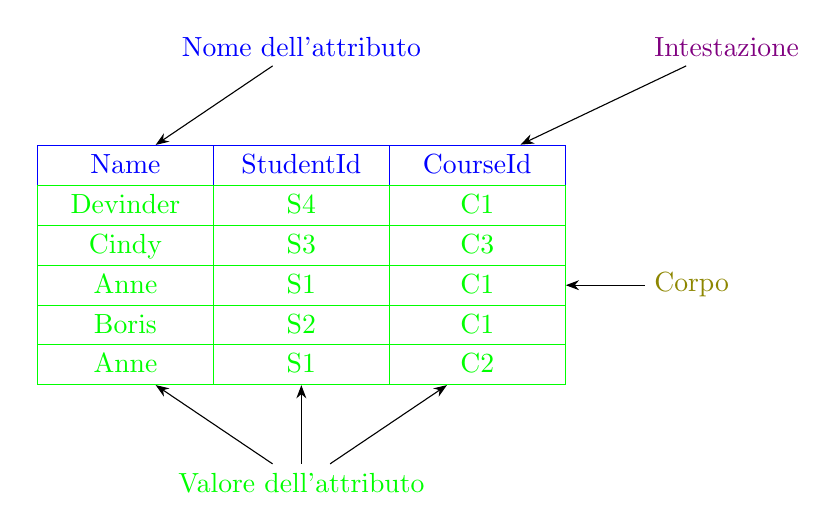
\begin{tikzpicture}
  % Stile per i nodi
  %\tikzstyle{every node}=[draw, rectangle, rounded corners]

  % Tabella
  \matrix (table) [
    every cell/.style= {nodes={text depth=0.2ex, text=green,draw=green,text width=2cm}},
    row 1/.style= {nodes={text depth=0.2ex, text=blue,draw=blue}},
    matrix of nodes,
    nodes={align=center},
    %column 1/.style={nodes={text width=2cm}},
    column sep=-\pgflinewidth,
    row sep=-\pgflinewidth]
  {
    Name & StudentId & CourseId \\
    Devinder & S4 & C1 \\
    Cindy & S3 & C3 \\
    Anne & S1 & C1 \\
    Boris & S2 & C1 \\
    Anne & S1 & C2 \\
  };

  % Annotazioni
  \node[above right=of table-1-3,text=violet] (header) {Intestazione};
  \node[right=of table-4-3,text=olive] (body) {Corpo};
  \node[below=of table-6-2,text=green] (attrVals) {Valore dell'attributo};
  \node[above=of table-1-2,text=blue] (attrName) {Nome dell'attributo};

  % Frecce
  \draw[-Stealth] (header) -- (table-1-3);
  \draw[-Stealth] (body) -- (table-4-3);
  \draw[-Stealth] (attrVals) -- (table-6-1);
  \draw[-Stealth] (attrVals) -- (table-6-2);
  \draw[-Stealth] (attrVals) -- (table-6-3);
  \draw[-Stealth] (attrName) -- (table-1-1);
\end{tikzpicture}
\end{document}
